\section{Lattice Theory}\label{lattice}
The static analysis we want to perform utilizes the mathematical theory of lattices together with a monotone function to guarantee that the analysis will terminate.
This theory will be described in the following.

\paragraph{Partial orders}
A lattice is a specialization of a partial order which will be described.
A partial order is a mathematical structure $L = (S, \sqsubseteq)$ where S is a set and $\sqsubseteq$ is a binary relation where the following conditions are satisfied:
\begin{itemize}
  \item Reflexivity: $\forall x \in S : x \sqsubseteq$
  \item Transitivity: $\forall x,y,z \in S : x \sqsubseteq y \wedge y \sqsubseteq z \Rightarrow x \sqsubseteq z$
  \item Antisymmetry: $\forall x,y \in S: x \sqsubseteq y \wedge y \sqsubseteq x \Rightarrow x = y$
\end{itemize}

\todo{maybe something about what this means and implications?}

\paragraph{Least upper bound}
As the name states, a least upper bound is the least of all upper bounds.
An upper bound y of a set X where $ X \subset S$ where S is a partial order is written as $X \subseteq y$.
y is an upper bound of X if we have that $\forall x \in X : x \sqsubseteq x$.

We can now define the least upper bound, written as $\sqcup X$:
\[X \sqsubseteq \sqcup X \wedge \forall y \in S : X \sqsubseteq y \Rightarrow \sqcup X \sqsubseteq y\]

The greatest lower bound $\sqcap X$ can be defined by the same logic.

\paragraph{Lattice}
A lattice can now be defined as a partial order in which $\sqcup X$ and $\sqcap X$ is defined for all $X \subset S$.
It should be noted  that a lattice must have a unique largest element $\top$ defined as $\top = \sqcup S$ and unique smallest element $\bot$ 

\begin{figure}
\begin{center}
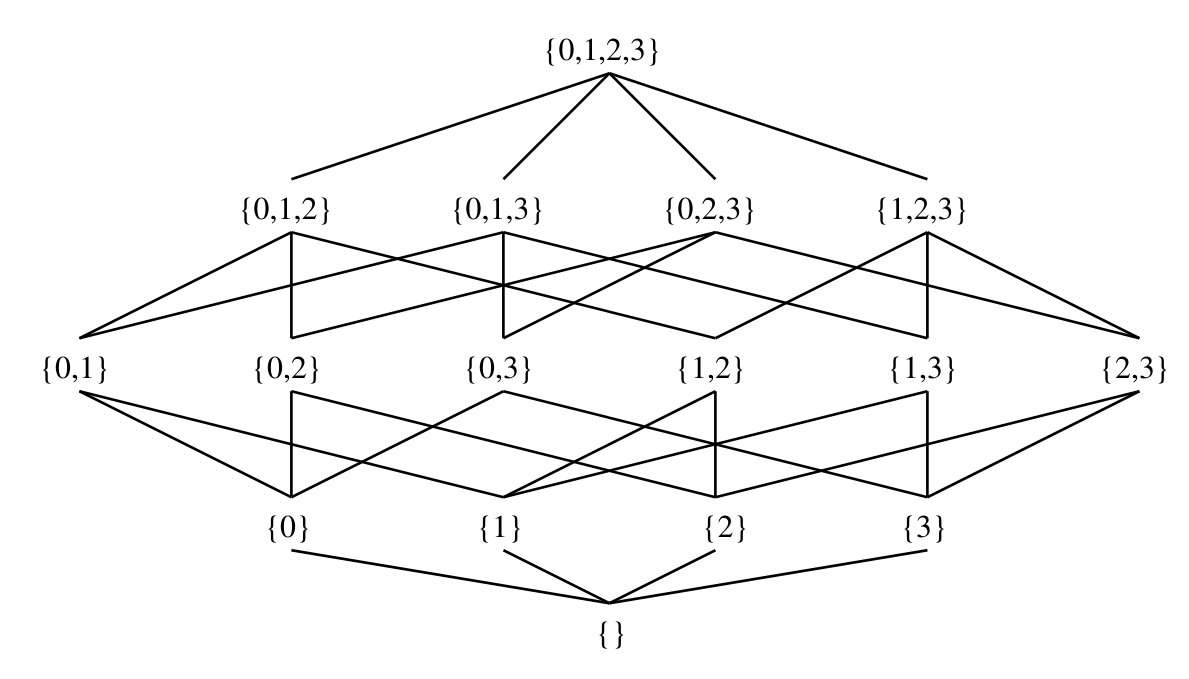
\includegraphics[width=0.7\textwidth]{figures/lattice_example_numbers}
\end{center}
\caption{A lattice with four elements}
\label{lattice_example}
\end{figure}

In \cref{lattice_example} a lattice with four elements is depicted.
This lattice is defined by the set $\{1, 2, 3, 4 \}$.
In general the set A defines a lattice $(2^A, \sqsubseteq )$ where $\top = \emptyset$, $\bot = A$, $x\sqcup y = x \cup y$ and $x \sqcap y = x \cap y$.

\todo{noget om hvordan vi vil bruge det i analysen? Synes det er svaert at skrive inden fixed point og analyserne er introduceret}
